\que{Адиабата Гюгонио и луч Михельсона.}

Пусть в совершенном газе есть поверхность разрыва, до разрыва газ
имеет макроскопические характеристики $\rho_1, p_1, u_1, e_1$, после разрыва -- $\rho_2, p_2, u_2, e_2$
(по обе стороны от разрыва находится одинаковый газ с одинаковыми определяющими соотношениями),
при этом материальные точки \textit{переходят} через поверхность разрыва: $M = \mathbf{D} \rho \neq 0$, где $\mathbf{D}$ -- скорость этой поверхности. 
Такую поверхность называют поверхностью ударной волны.

Положим $C_{n\Sigma} = C_{3\Sigma} = 0$, введём удельные объёмы
$V_1 = 1 / \rho_1, V_2 = 1 / \rho_2$. Тогда соотношения Гюгонио можно записать в виде:
\[
  \begin{cases}
    \dfrac{u_1}{V_1} = \dfrac{u_2}{V_2}, \\
    \dfrac{u_1^2}{V_1} - \dfrac{u_2^2}{V_2} = p_2 - p_1, \\
    e_1 - e_2 = \dfrac{u_2^2 - u_1^2}{2} + p_2 V_2 - p_1 V_1.
  \end{cases}
\]
Пусть значения после разрыва будут известными, тогда выразим значения до разрыва:
\[
  \begin{cases}
    u_1 = \dfrac{V_1 u_2}{V_2}, \\
    u_2^2 \dfrac{V_1}{V_2^2} - \dfrac{u_2^2}{V_2} = p_2 - p_1 \Rightarrow \dfrac{u_2^2}{V_2^2} = \dfrac{p_2-p_1}{V_1 - V_2},
  \end{cases}
\]
тогда
\[
  \begin{cases}
    u_2 = \pm V_2 \sqrt{\dfrac{p_2-p_1}{V_1 - V_2}}, \\
    u_1 = \pm V_1 \sqrt{\dfrac{p_2 - p_1}{V_1 - V_2}}
  \end{cases}
\]
найдём тогда скачок внутренней энергии:
\[
  [e] = e_2 - e_1 = p_1 V_1 - p_2V_2 + \dfrac{u_1^2 - u_2^2}{2} =
  \dfrac{p_2-p_1}{V_1-V_2} \dfrac{V_1^2 - V_2^2}{2} + p_1V_1 - p_2V_2 =
  \dfrac{1}{2} (p_1+p_2) (V_1 - V_2)
\]
полученное выражение называется \emph{адиабатой Гюгонио} (или \emph{ударной адиабатой}).

Если известны $e_i (p_i, V_i)$, то адиабата Гюгонио связывает между собой давление и удельный
объём с одной и с другой стороны поверхности раздела, т.е. если с одной из сторон разрыва
газ принимает значения $(p_1, V_1)$, то с другой стороны газ может принимать множество разных
значений $(p_2, V_2)$, но обязательно лежащих на этой кривой.

\paragraph{Адиабата Гюгонио для совершенного газа.}
Стоит отметить, что в случае совершенного газа $e = \tilde e_0 + \dfrac{pV}{k-1}$,
тогда в случае совершенного газа (пусть нет скачка начальной внутренней энергии $\tilde e_0$):
\[
  \dfrac{p_2V_2 - p_1V_1}{k-1} = \dfrac{1}{2} (p_1+p_2) (V_1 - V_2).
\]
\begin{figure}[H]
  \centering
  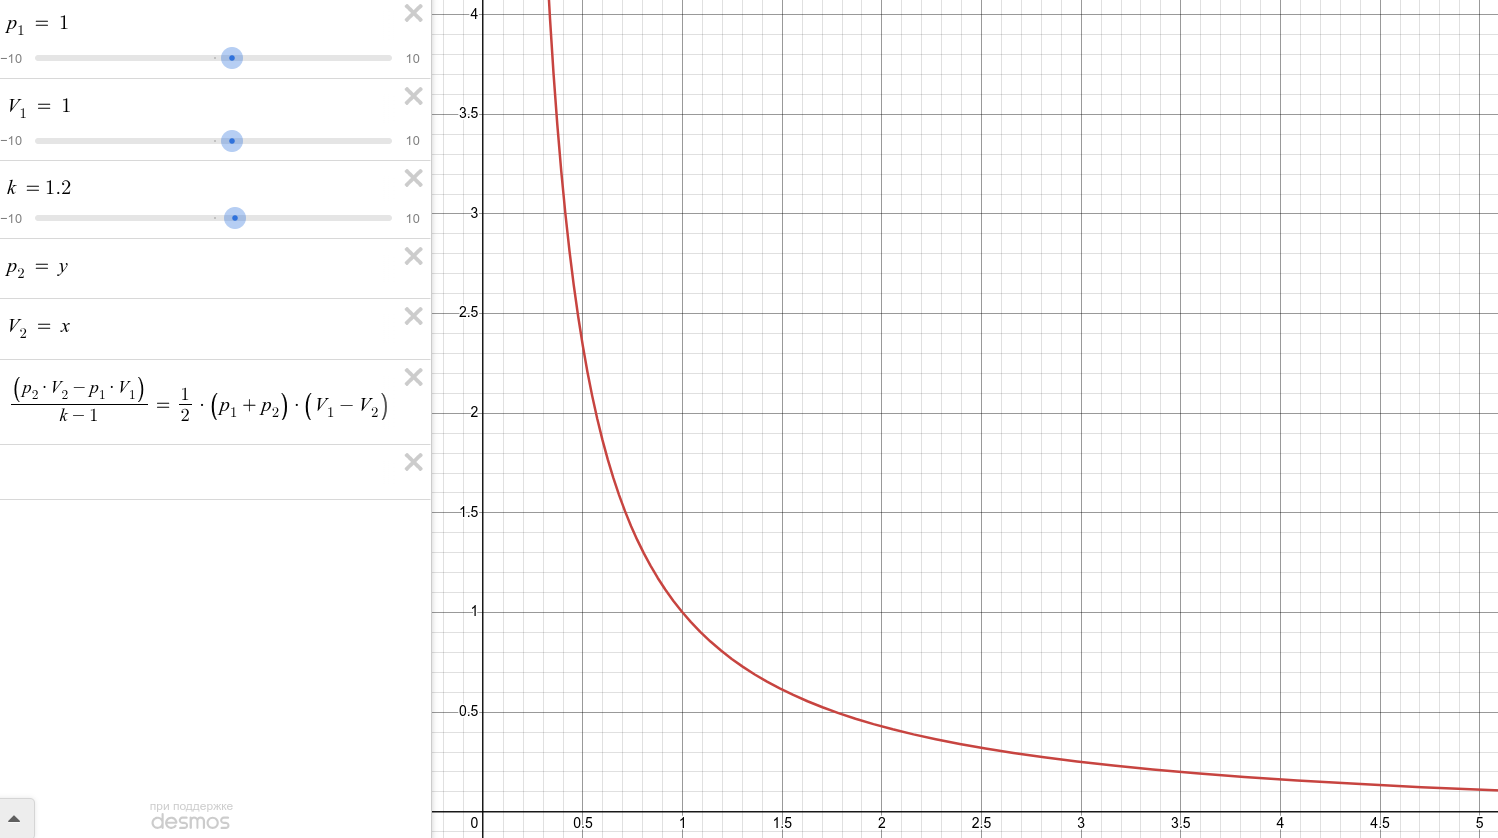
\includegraphics[width=0.9\linewidth]{img/Gugonio_adiabata_desmos.png}
  \caption{Адиабата Гюгонио для совершенного газа при адиабатических процессах. Фото в цвете}
\end{figure}

\paragraph{Доказательство невозрастания.}
Адиабата Гюгонио всегда (при любых фиксированных $(p_1, V_1)$) невозрастает. 
\begin{proof}
  Для доказательства этого покажем, что любая секущая, проходящая через
  точку $(p_1, V_1)$ и точку $(p_2, V_2)$ невозрастает.
  Уравнение секущей: $p - p_1 = \tg \alpha \cdot (V - V_1)$, 
  а $\tg \alpha$ можно найти из выражения для $u_2 = \pm V_2 \sqrt{\dfrac{p_2-p_1}{V_1 - V_2}}$:
  \[
    \tg \alpha  = \dfrac{p_2 - p_1}{V_2 - V_1} = - \dfrac{u_2^2}{V_2} \leqslant 0
  \]
  Таким образом, любая секущая невозрастает, а значит и сама адиабата невозрастает.
\end{proof}

Построенная секущая называется \emph{лучом Михельсона} (также Релея) (луч, потому что $p \geqslant 0$).
